\documentclass[10pt]{article}
\usepackage[spanish]{babel}
\usepackage[utf8]{inputenc}
\usepackage{graphicx} 
\title{M\'etodos abiertos, M\'etodo de la secante}
\author{R\'omulo Walter Condori Bustincio}
\date{}
\begin{document}
\maketitle
\begin{enumerate}
\item para el an\'alisis, se considera la siguiente funci\'on $$x^2- 2$$, cuya gr\'afica es la siguiente:
\begin{center}
 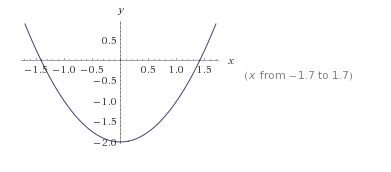
\includegraphics[scale=0.8]{./grafica.jpg}
 % grafica1.jpg: 0x0 pixel, 300dpi, 0.00x0.00 cm, bb=
\end{center}
el algoritmo produce la siguiente salida:\\

Con un total de 4 de 100 iteraciones permitidas, se obtuvo la siguiente tabla:
\begin{center}
\begin{tabular}{|c|c|c|}
\hline
Iteraci\'on&$r$&$f(r)$\\
\hline
0&2&-1\\
1&1.33333&2\\
2&1.4&-0.222222\\
3&1.41463&-0.04\\
4&1.41421&0.00118977\\
\hline
\end{tabular}
\end{center}
Donde el valor de $r$ aproximado es 1.41421 con un error relativo de: 2.12358e-06

\end{enumerate}
\end{document}

